%----------------------------------------------------------------------------------------
%	6./ Beam Pattern
%----------------------------------------------------------------------------------------
%\section{Beam Pattern}
%\label{se:beam}

The NIKA2 beam pattern mainly depends on the IRAM \trentemetre\ telescope and
NIKA2 full (external and internal) optical system characteristics,
whereas the detectors themselves might have an impact at sub-dominant
level (through \emph{e.g.} time constants or correlated noises).
The full beam pattern is characterized using \bm\ observations. First,
we produce deep integration maps of bright sources to provide a
qualitative description of the complex beam structure in
Sect.~\ref{se:fullbeam}. Then we model the beam using three
complementary methods to estimate the main beam angular resolution
(Sect.~\ref{se:mainbeam}) and the beam efficiency
(Sect.~\ref{se:beam_efficiency}).

\subsection{Full beam pattern}
\label{se:fullbeam}

We present the two-dimensional pattern of the beam in
Fig.~\ref{fig:features}. We primarily use a map obtained from a combination
of \bm\ observations of strong point sources collected during
N2R8 and N2R9 technical campaigns. Namely, we use \bm\ scans
of Uranus%(scan id '20170125s223' and '20170125s243')
,  Neptune %('20170224s177')
and the bright quasar 3C84. %('20170226s415').
However, we checked the stability of our results on single scan maps,
combinations of scans for a single source, and combinations of
shallower scans but spanning a large range of scanning direction.
%The data processing includes a mitigation of the correlated noise, which
%mainly originates from the atmosphere.  We primarly use a subtraction
%of a common mode estimated from the most correlated detectors (the
%so-called 'cm one block' method). However, other methods are tested
%for assessing the immunity of our results to noise residuals.

%\begin{figure}[!thbp]
%\begin{center}
%  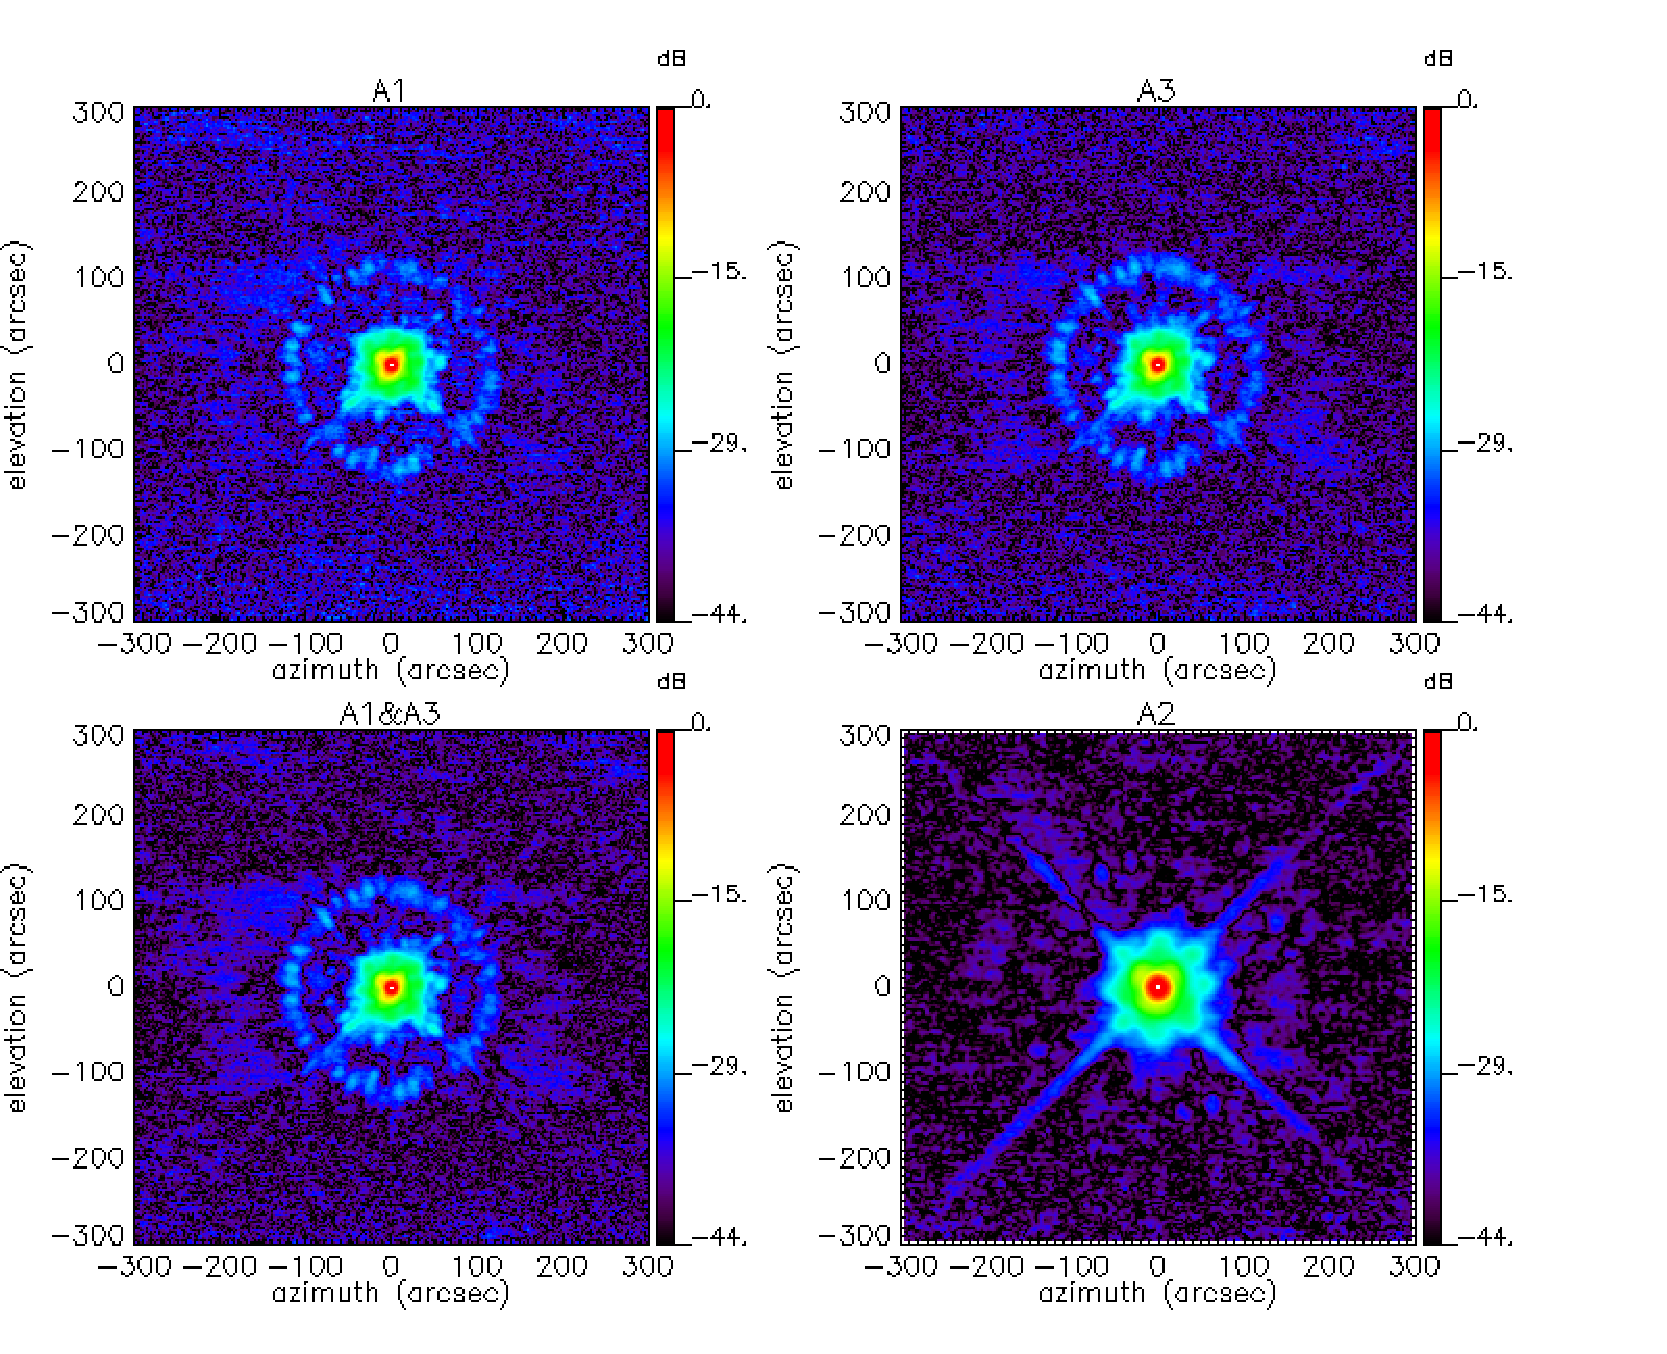
\includegraphics[trim=0cm 0cm 2.5cm 0cm, clip=true, width=\linewidth]{Figures/Lobe_map_Combo_v2_dB.pdf}
% \caption[Beam pattern.]{From upper left to lower right, beam maps of array 1 (labeled 'A1'), array 3 ('A3'), the combination of the $1\,\rm{mm}$ arrays ('A1$\&$3') and the  $2\,\rm{mm}$ array ('A2') are shown in decibel. These maps, which consist of normalized combination of four long OTF scans of bright point sources, are in horizontal coordinates and cover a sky area which extends over 10 arcmin.}
%\label{fig:beam}
%\end{center}
%\end{figure}

\begin{figure}[!thbp]
\begin{center}
  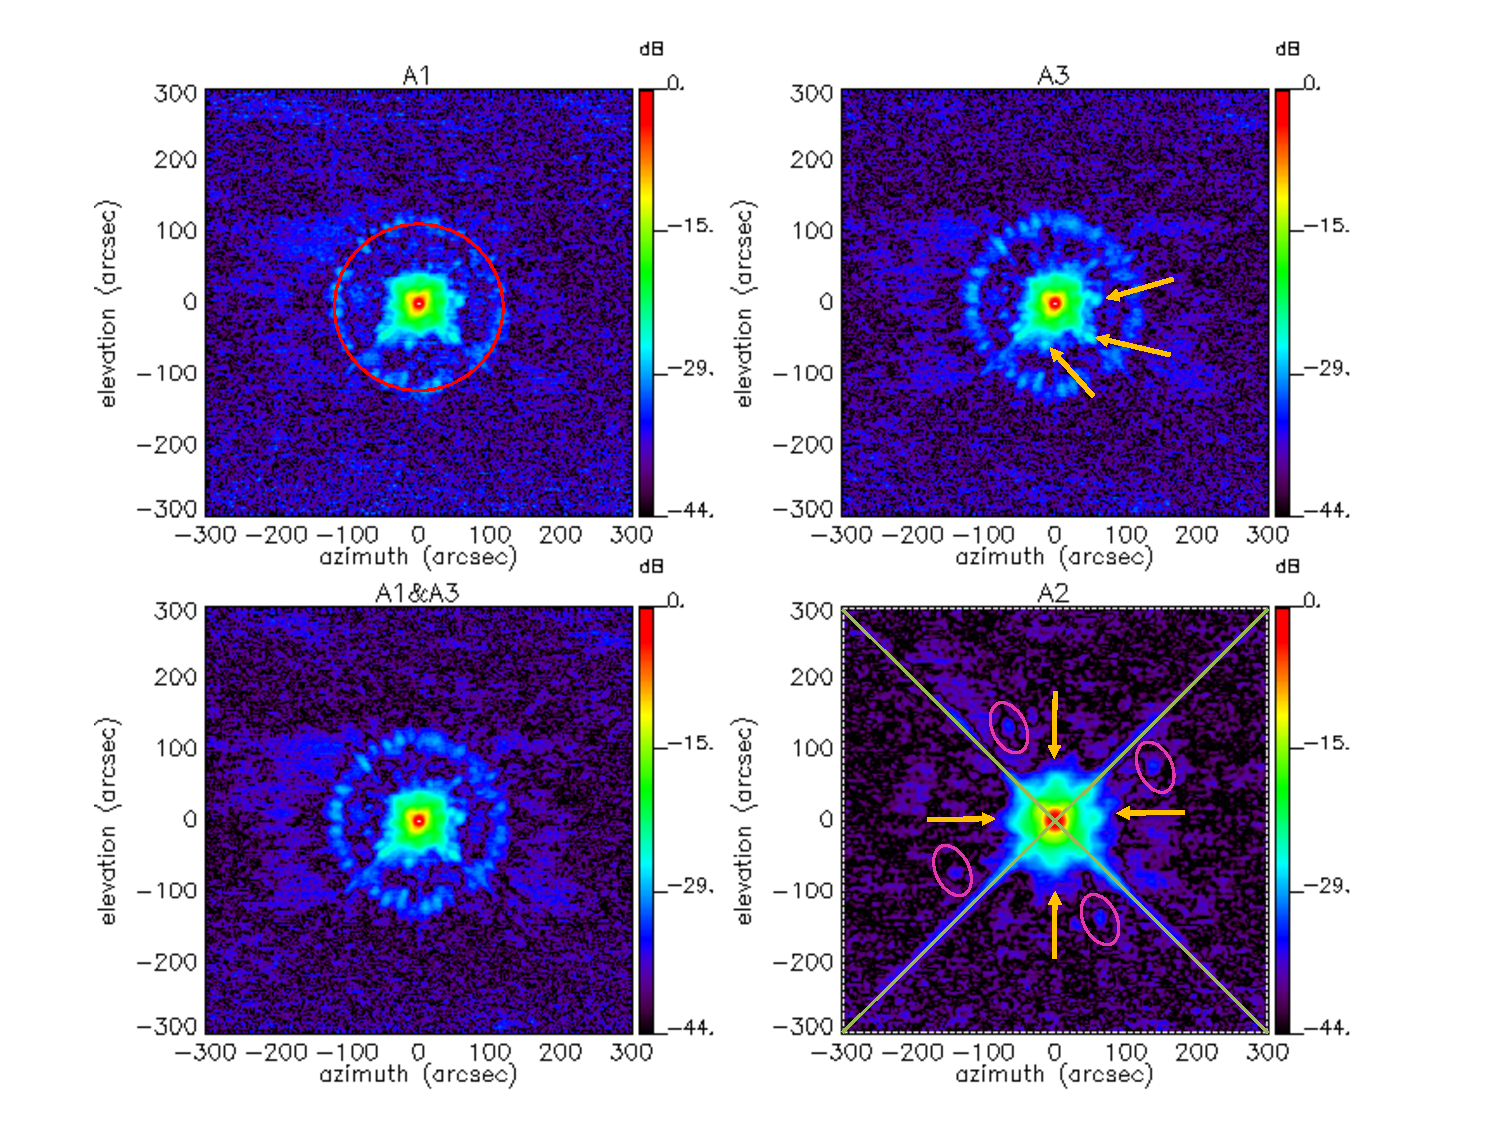
\includegraphics[trim=0.5cm 0.5cm 1cm 0cm, clip=true, width=\linewidth]{Figures/Beams_features.pdf}
\caption[Noticeable features of NIKA2 beam pattern.]{From upper left
  to lower right, beam maps of array 1 (labeled 'A1'), array 3 ('A3'),
  the combination of the $1\,\rm{mm}$ arrays ('A1$\&$3') and the
  $2\,\rm{mm}$ array ('A2') are shown in decibel. These maps, which
  consist of normalized combination of four long OTF scans of bright
  point sources, are in horizontal coordinates and cover a sky area
  which extends over 10 arcmin. %Same maps as in Fig.~\ref{fig:beam}
  %with some noticeable features.
  The solid lines and arrows highlight some noticeable features.
  Red circle in the
  A1 map (upper left panel): diffraction ring seen in 1-mm maps
  (the spokes are presumably caused by radial and azimuthal panel buckling (cf. Fig.4 in Greve et
  al. 2010)); Orthogonal green lines in the A2 map (lower right panel): diffraction
  pattern caused by quadrupod secondary support structure (prominently
  seen in A2 map); Yellow arrows in the A3 map (upper right panel):
  pattern of 3 spikes seen in 1mm maps of unknown origin; Yellow
  arrows in A2 map (lower right panel): four symmetrical spikes of the
  first sidelobes; Pink ellipses: 4 spikes seen in A2 maps.}
\label{fig:features}
\end{center}
\end{figure}

The deep NIKA2 beam maps reveal some noticeable features, which are
shown in Fig.~\ref{fig:features}. Ranging from strong and/or extended to
weak and/or spiky, they include:
\begin{itemize}
\item[(1)] the main beam and the underlying first error
  beam, which is due to the large scale deformations of the primary
  mirror, and the first side lobes. The latter include 
  the 20" diameter first side lobe and the 60" diameter (squarish)
  side lobe, which is due to the convolution of the primary mirror and quadrupod
  diffraction pattern with the pixel transfert function;
  %The four symmetrical spokes of the error beam as shown by
  %yellow arrows in the A2 panel, are expected from ZEMAX
  %simulations;
\item[(2)] the diffraction ring by panel buckling of the primary
  mirror, as shown with a red circle in the A1 panel;
\item[(3)] the side lobes shown with green
  diagonal lines in the A2 panel are due to diffraction on the
  quadrupod holding the secondary mirror of the telescope, as expected
  from ZEMAX simulations;  
\item[(4)] spikes of not fully understood origin pointed with yellow
  arrows. The ones that are along the vertical and
  horizontal axes are reproduced by ZEMAX simulation but at a 
  shallower level, whereas the ones shown in the A3 panel in the
  diagonal directions may be due to the small cylindrical
  instrumentation box on the side of the M2 cabin. The origin of the
  asymmetry on the 1~mm arrays is unknown but most probably due to
  internal optics aberrations;
\item[(5)] shallow spikes of unknown origin, which are circled by pink
  ellipses. The multiple images on the combined deep beam map indicate
  a rotation of these spikes with the observing elevation, which in
  turn point to diffraction related issue or a ghost image that are
  formed inside the cryostat. These shallow features are expected to
  have no sizable impact on the science-purpose map of NIKA2.
\end{itemize}

We further quantify the respective level of the axi-symmetrical
features of the beam pattern in evaluating the beam radial profile
$B(r)$, which is the normalised radial brightness profile,
where $r$ is the radius from the beam center.
%is the azimuthal average of the beam map around the
%main beam center.
Although the profile cannot represent the sub-dominant non-axisymmetrical
features, which are seen in Fig.~\ref{fig:features} (quadrupod
diffraction pattern, spikes), it provides us with a useful
representation of the internal and central parts of the beam (about up to
$100''$). We determine a beam profile from a beam map in centering to
the fitted value of the main beam center and in forming the
weighted average of the map pixels in annular rings.

We checked the stability of the beam against various observing
conditions (source intensity, weather condition, focus optimisation) by
comparing the beam profiles of a series of \bm\ observations.
This \bm\ set has been selected from all the available \bm\ scans at
optimal focus using the baseline selection criteria, as given in
Sect.~\ref{se:data_selection}.
%The 18 beam profiles and their difference w.r.t. the median beam
%profile are shown in Fig.~\ref{fig:beam_prof}.
The 18 beam profiles are shown in
Fig.~\ref{fig:beam_prof}. Calculating the difference of the beam
profiles to the median beam profile, we find a dispersion below $5\%$ at
$1\,\rm{mm}$ and below $2\%$ at $2\,\rm{mm}$. 

%%%%%%%%%%%%%%%%%%%%%%%%%%%%%%%%%%%%%%%%%%%%%%%%%%%%%%%%%%%%%%%%%
% Stability of the beam pattern
\begin{figure}[!thbp]
  \centering
%   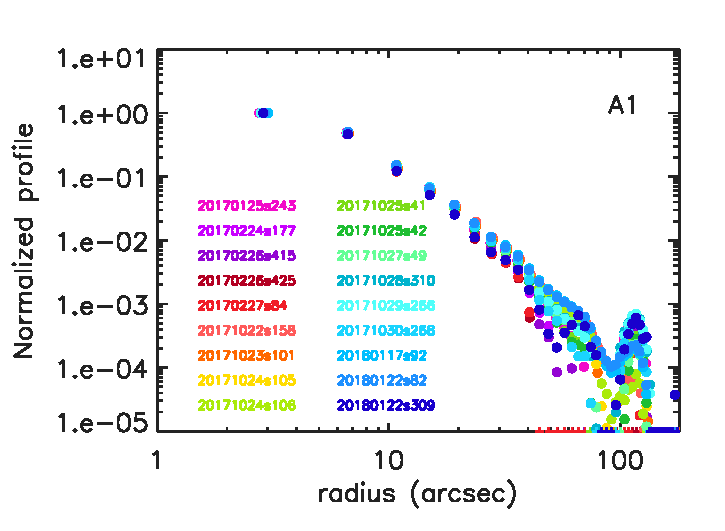
\includegraphics[clip, width=0.42\textwidth]{Figures/Beams/plot_profiles_a1.pdf}
%   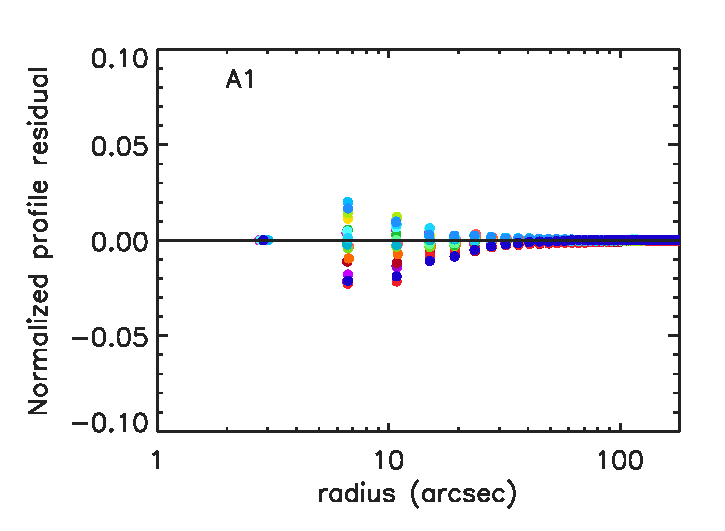
\includegraphics[clip, width=0.42\textwidth]{Figures/Beams/plot_profile_diff_wrt_median_a1.pdf}
%   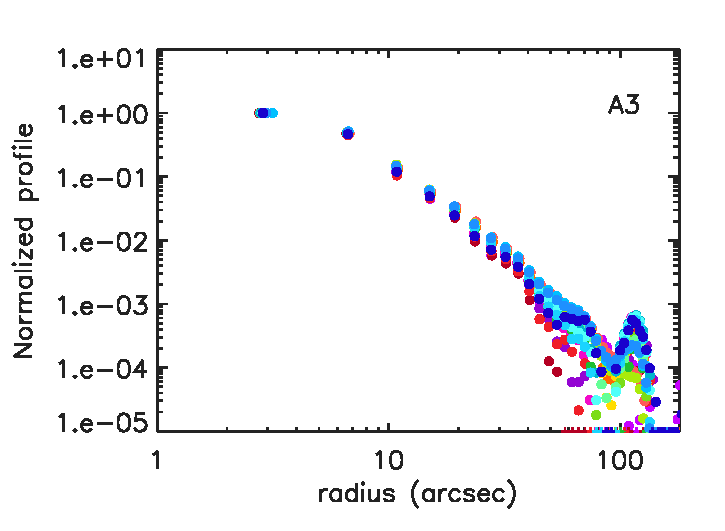
\includegraphics[clip, width=0.42\textwidth]{Figures/Beams/plot_profiles_a3.pdf}
%   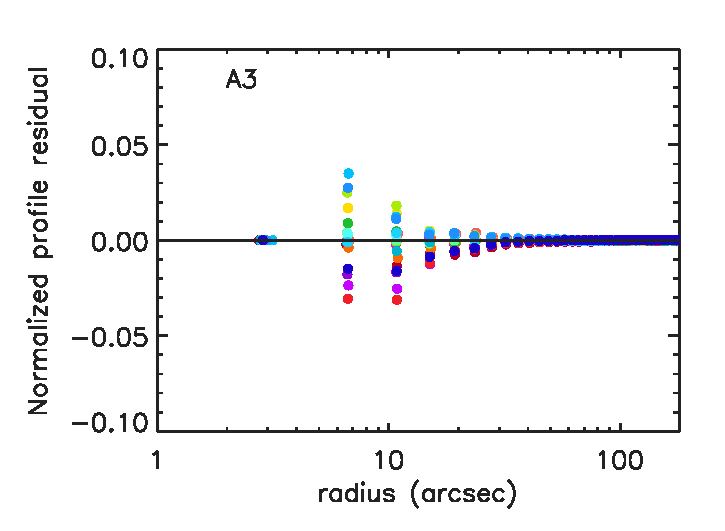
\includegraphics[clip, width=0.42\textwidth]{Figures/Beams/plot_profile_diff_wrt_median_a3.pdf}
   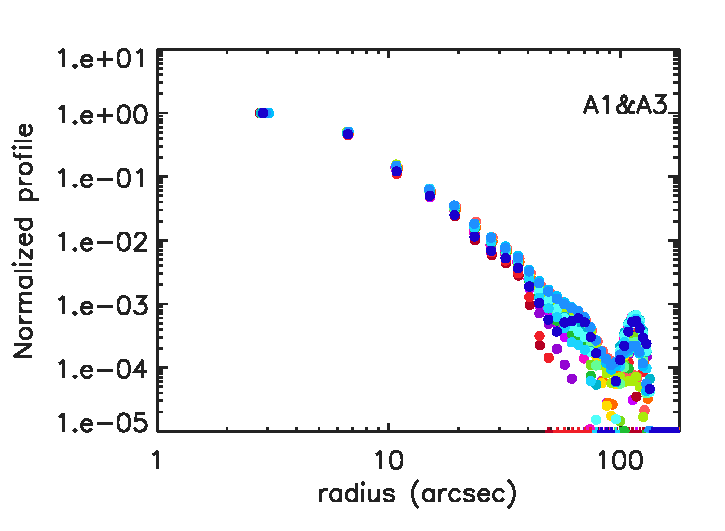
\includegraphics[clip, width=\linewidth]{Figures/plot_profiles_1mm.pdf}
%   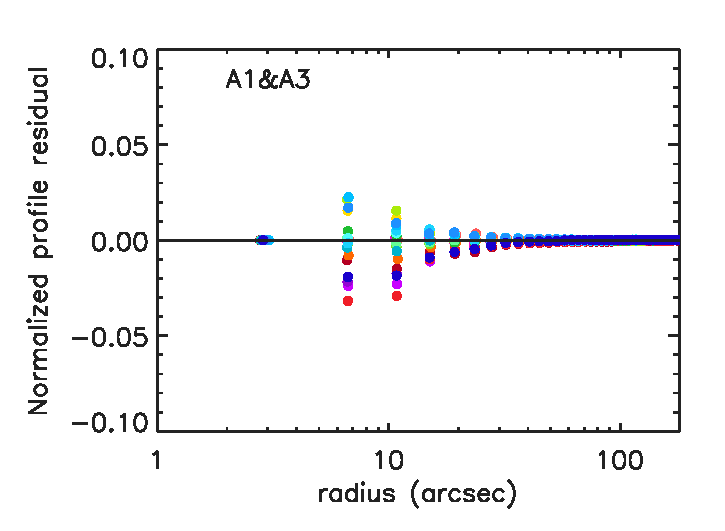
\includegraphics[clip, width=\linewidth]{Figures/plot_profile_diff_wrt_median_1mm.pdf}
   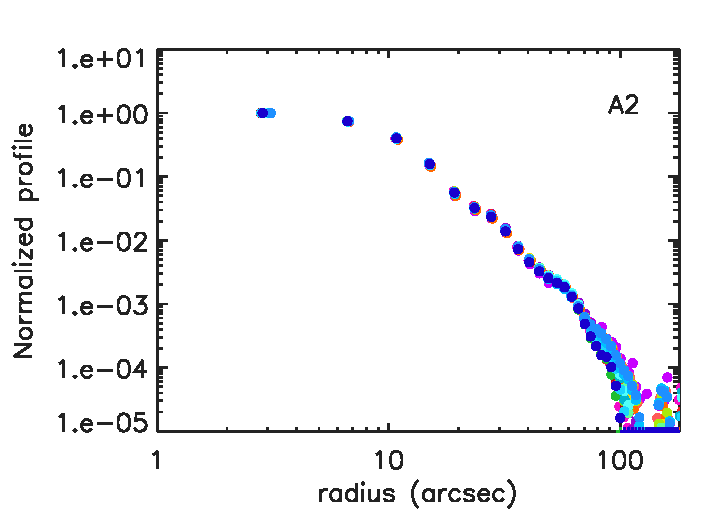
\includegraphics[clip, width=\linewidth]{Figures/plot_profiles_a2.pdf}
%   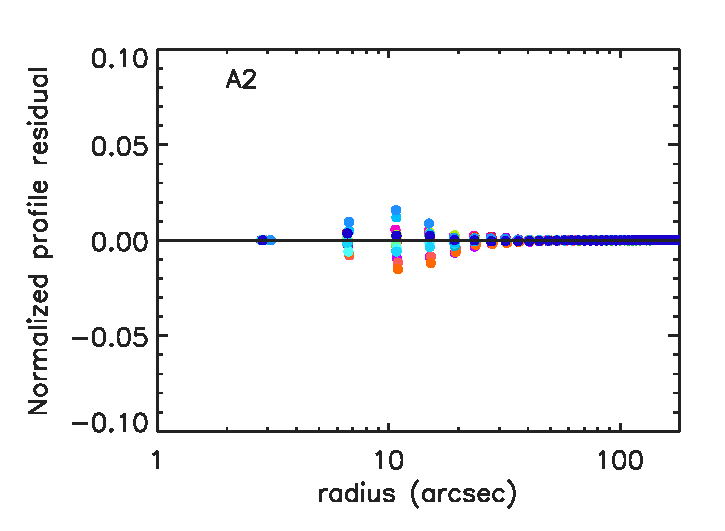
\includegraphics[clip, width=\linewidth]{Figures/plot_profile_diff_wrt_median_a2.pdf}
  \caption[Stability of the beam profile]{Beam radial profiles as a
    function of the radius from the peak for a series of 18
    \bm\ scans acquired during the N2R8 and N2R9 calibration campaigns and
    during the N2R12 and N2R14 science pools.}
    %Left column plots: 
    %Beam profiles normalised to the maximum value; Right column plots:
    %difference w.r.t. the median normalised profile.
    %The radial
    %profile shapes are stable at better than $5\%$ 
    %against observing conditions.}
  \label{fig:beam_prof}
\end{figure}


%An example of the beam profile from a beam map acquired during {\emph N2R8} (scan ID:
%20170125s243)\todo{verifier le scan utilise pour les figures,
%  possibilite que ce soit 20170125s223 pris l'apres-midi}, as well as the best-fit 3-Gaussian model, is shown in
%the right panels of Fig.~\ref{fig:beam_structure_example}.

%We further fit the three-Gaussian model of Eq.~\ref{eq:3gauss} to each
%profile and gather the average best-fitting amplitudes with respect to
%the peak amplitude and FWHM in Table~\ref{tab:mean_3gauss_fit}. The
%errors are evaluated as the standard deviation of the best-fitting
%parameter values of the 18 \bm\ scans, and thus do not account for the
%correlation between parameters. These values are given to gain insight
%of the axisymmetrical pattern of the beam, but are not further used for
%the calibration. 
%
% AVERAGE 3-GAUSSIAN FIT
%\begin{table}[th]
%  \begin{center}
%    \begin{tabular}{|c|c|c|c|c|c|c|}
%      \hline
%      & \multicolumn{6}{|c|}{3-Gaussian profile parameters}  \\\cline{1-7}
%      Arrays       & Amp 1 & Amp 2 & Amp 3 & FWHM 1 & FWHM 2 & FWHM 3 \\
%      \hline\hline
%      A1        &  $0.89 \pm 0.01$   &  $0.08 \pm 0.02$  & $5 \times 10^{-3} \pm 2 \times 10^{-3}$  &  $11.0 \pm 0.2 $ & $29 \pm 2 $  & $65 \pm 15 $ \\  
%      A3        &  $0.90 \pm 0.01$   &  $0.07 \pm 0.01$  & $4 \times 10^{-3} \pm 2 \times 10^{-3}$  &  $11.0 \pm 0.2 $ & $30 \pm 3 $  & $72 \pm 23 $ \\  
%      1mm       &  $0.90 \pm 0.01$   &  $0.07 \pm 0.01$  & $4 \times 10^{-3} \pm 2 \times 10^{-3}$  &  $11.0 \pm 0.2 $ & $29 \pm 2 $  & $70 \pm 15 $ \\  
%      2mm       &  $0.96 \pm 0.01$   &  $0.3 \pm 0.3$    & $1 \times 10^{-3} \pm 0.3$ &  $17.5 \pm 0.1 $ & $63 \pm 10 $ & $65 \pm 12 $ \\  
%      \hline\hline
%    \end{tabular}
%    \caption[Average 3-Gaussian beam profile parameters]{Average
%      3-Gaussian beam profile parameters. The FWHMs are given in arcseconds.}
%    \label{tab:mean_3gauss_fit}
%  \end{center}
%\end{table}



\subsection{Main beam}
\label{se:mainbeam}

NIKA2 angular resolution depends on the angular size of the main beam,
defined as the principal Gaussian (of the smaller FWHM) that encloses
most of the measured point-like source flux density. We developped
three methods for the main beam characterisation, which are detailed
in Sect.~\ref{se:mainbeam_methods}. Sect.~\ref{se:mainbeam_dataset}
presents the observing scans that we have selected to derive the results
discussed in Sect.~\ref{se:mainbeam_results}. We check the stability
of the FWHM estimate against the observing conditions in
Sect.~\ref{se:mainbeam_stability}.


\subsubsection{Main beam characterization methods}
\label{se:mainbeam_methods}
To characterize the main beam and derive an estimate of the FWHM, we
have developped three methods. The two first methods, quoted
{\tt Prof 1\&2}, rely on a fit
of the beam profile to benefit from the signal-to-noise ratio increase
after azimuthally averaging the signal. The last one by contrast,
consists in an elliptical Gaussian fit of the beam map for a better
2D modeling, and is labeled {\tt 2D beam}. They are presented in more
detail below. \\

\noindent {\tt Prof 1}: We fit the beam profile using an empirical function,
which accounts for both the main beam and the error beams and side
lodes, and derive the FWHM from the main beam parameter. The beam
profile $B(r)$ is modeled using a three-Gaussian function defined as:
\begin{equation}
  B(r) = \sum_{i=1}^{3} \mathcal{A}_i G_i(r) + \mathcal{B}_0,
  \label{eq:3gauss}
\end{equation}
where $\mathcal{A}_i$ is the amplitude of the Gaussian $i$ for $i \in {1, 2, 3}$ and
$\mathcal{B}_0$ a pedestal level accounting for the residual noise
level in the map. The FWHM estimate is given by the best-fitting value
of the FWHM for the first Gaussian function.\\

\noindent {\tt Prof 2}: A single Gaussian is fit to the beam profile after
masking the portion of the profile where the contributions of the side
lobes and error beams are the largest. Specifically, the side lobe mask
is designed to cut out the radius comprized between $0.65\, $FWHM$_0$,
where FWHM$_0$ is the reference Gaussian beam FWHM (see
Sect.~\ref{se:photometric_system}) and $80''$. At radial distances
greater than $80''$, the profile measurement provides the base level
for the Gaussian fit. The profile is estimated up to a radius of
$180''$, that is in the inner part of the beam map where the noise
variance is uniform.\\

\noindent {\tt 2D beam}: We model the two-dimensional distribution of the main
beam using an elliptical Gaussian. We characterize NIKA2 resolution
by forming the \emph{FWHM}, defined as
\begin{equation}
  FWHM = 2 \sqrt{2\ln {2}\, \sigma_x\sigma_y},
\end{equation}
where $\sigma_x$ and $\sigma_y$ are the Gaussian standard deviation
along minor and major axis.
As in {\tt Prof 2}, we use masked versions of the
beam map to avoid the side lobe and error beam contaminations.
The mask consists in cutting an annulus of inner radius
$r_{\rm{in}}$ and outer radius $r_{\rm{out}}$ centered on the beam
maximum. Whereas $r_{\rm{out}}$ is conservately set to be $100''$,
$r_{\rm{in}}$ is let free to vary around a central value about $8''$
for A1 and A3 and about $12''$ for A2 to provide the best 2D Gaussian
fit.

\subsubsection{Main beam data sets}
\label{se:mainbeam_dataset}

We select a sub-set of the \bm\ scan selection described in
Sect.~\ref{se:fullbeam} by discarding scans of Mars.
The 12 remaining \bm\ scans are analysed using the data reduction
pipeline of Sect.~\ref{se:dataproc} and projected onto maps
with a resolution of $1''$ and an angular size of $10'$.

We also consider a series of shorter integration scans. We select $5'x8'$ OTF
scans of moderately bright to very bright point sources by
thresholding the flux density estimates at $1~\rm{Jy}$ at both
wavelengths. Slightly extended sources, such as Mars, NGC7027 and
CRL2688 are discarded. After the baseline selection cuts, as described in
Sect.~\ref{se:data_selection}, the data set comprises 154 %163
scans
towards the giant planets Uranus and Neptune, the secondary calibrator
MWC349 and the quasars 3C84, 3C273, 3C345 and 3C454 (aka
2251+158). The data are reduced and projected onto $2''$ resolution
maps. 

\subsubsection{Results}
\label{se:mainbeam_results}

We have derived the main beam FWHM for the three arrays and the
$1\,\rm{mm}$ arrays combination using the three methods presented in
Sect.~\ref{se:mainbeam_methods} and the data
sets of Sect.~\ref{se:mainbeam_dataset}. Namely, our main beam FWHM estimates
consist of i) the median FWHM estimate using {\tt Prof 1} from the 12 \bm\ scan
sub-set, ii) the average FWHM estimate using {\tt Prof 2} on a series
of \bm\ and $5' \times 8'$ OTF scans of Uranus and Neptune, the {\tt 2D beam} average FWHM
from iii) the series of OTF scans described in
Sect.~\ref{se:mainbeam_dataset} and iv) from the 12 \bm\ scan
sub-set. By comparing these results, we test the stability of the FWHM
estimates against the choices of the data set and of the estimation
method. %We also seek at validating the FWHM estimates using
%{\tt Prof 2}, which is further used to derive the beam efficiency in
%Sect.~\ref{se:beam_efficiency}.

For Uranus, the
FWHM estimates are further corrected for the beam broadening due to the
extension of the apparent
disc. At the IRAM $30\,\rm{m}$ latitude, Uranus disc diameter varies
from $3.3''$ to $3.7''$. This induces a broadening of the Gaussian main beam of
$0.19 \pm 0.03\,\rm{arcsec}$ at $1\, \rm{mm}$ and $0.12 \pm 0.02\,\rm{arcsec}$
at $2\, \rm{mm}$. Uranus FWHM estimates are corrected for the average beam
widening values.

The results of this analysis are
gathered in Table~\ref{tab:fwhm}, including error bars evaluated as
the rms dispersion of single-scan based FWHM estimates.
All the tests based on {\tt Prof 2} and {\tt 2D beam}, which both
resort to a sidelobe mask, yield FWHM estimates
in agreement within error bars, whereas the test using {\tt Prof 1}
yields slightly smaller FWHM for all arrays.
The latter provides us with lower limits for the main beam FWHM.
The error bars are the most robustly derived from the dispersion of the
best-fitting FWHM over the set of 154 OTF scans, whereas rms errors
that are estimated from smaller and more homogeneous scan sets are likely to be
underestimated. The combined results are obtained from an error-weighted
average of the four FWHM estimates for each array. The 12 \bm\ scan
based rms errors were replaced by the 154 OTF scan based rms errors
beforehand. The combined results, as given in
Table~\ref{tab:fwhm}, provide us with a robust evaluation of the
FWHM. Hence, we report FWHMs of $11.1''\pm0.1''$ at
$1\, \rm{mm}$ and $17.6''\pm 0.1''$ at $2\, \rm{mm}$.  

\begin{table*}[!thbp]
  \caption[]{Estimates of the main beam FWHM in arcsec, using three estimation methods (see
    Sect.~\ref{se:mainbeam_methods}) and three data sets
    (see Sect.~\ref{se:mainbeam_dataset}), and their combination.}
  \label{tab:fwhm}
  \centering
  \begin{tabular}{llrrrr}
    \hline\hline
    \noalign{\smallskip}
%       &    &  \multicolumn{4}{c}{Array or array combination} \\
%    \cline{3-6}
    Method & Dataset        &   A1 &  A3 & A1 $\&$ A3 &  A2  \\
    \noalign{\smallskip}
    \hline
    \noalign{\smallskip}
    {\tt Prof 1}  &  \bm\     & $10.8 \pm 0.1$  &  $10.8 \pm 0.1$  & $10.8 \pm 0.1$  &  $17.4 \pm 0.1$  \\
    {\tt Prof 2}  &  mixed    & $11.3 \pm 0.4$  &  $11.2 \pm 0.4$  & $11.2 \pm 0.3$   & $17.4 \pm 0.2$  \\ 
    {\tt 2D beam} &  5x8 OTF  & $11.3 \pm 0.2$  &  $11.1 \pm 0.2$  & $11.2 \pm 0.2$  &  $17.8 \pm 0.1$  \\ 
                  &  \bm\     & $11.2 \pm 0.1$  &  $11.1 \pm 0.1$  & $11.2 \pm 0.1$  &  $17.6 \pm 0.1$  \\
    \noalign{\smallskip}
    \hline
    \noalign{\smallskip}
    \multicolumn{2}{c}{Combined}               & $11.1 \pm 0.2$  & $11.0 \pm 0.2$  & $11.1 \pm 0.2$  &  $17.6 \pm 0.1$  \\
    \noalign{\smallskip}
    \hline
  \end{tabular}
\end{table*}

\subsubsection{Stability checks of the main beam}
\label{se:mainbeam_stability}

\begin{figure}[!thbp]
\begin{center}
  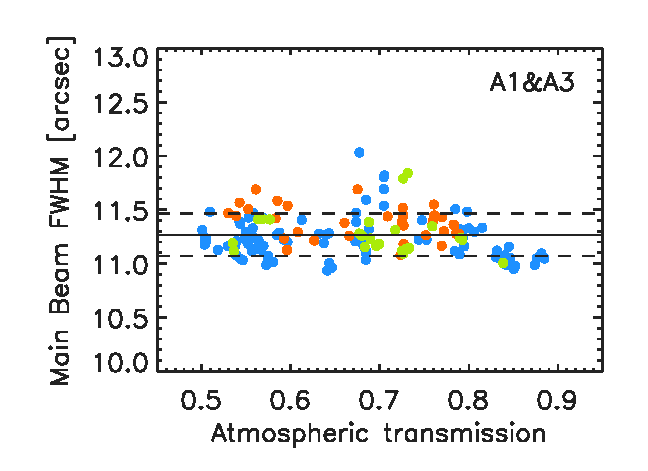
\includegraphics[clip, width=0.45\textwidth]{Figures/plot_FWHM_vs_atmtrans_mb_radius_binning2_1mm.pdf}
  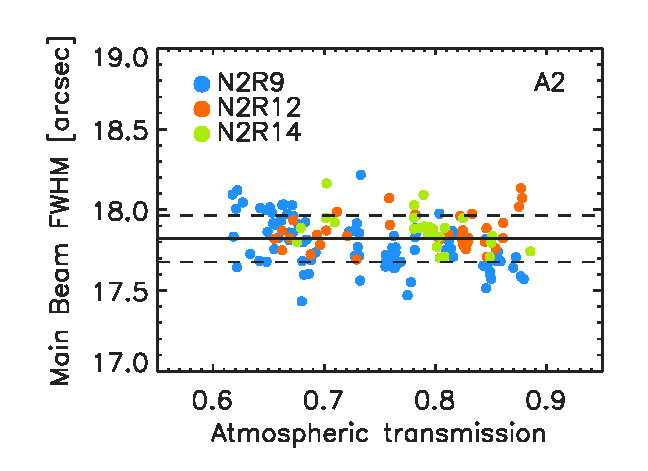
\includegraphics[clip, width=0.45\textwidth]{Figures/plot_FWHM_vs_atmtrans_mb_radius_binning2_a2.pdf}
  \caption[Main Beam FWHM]{Main beam FWHM estimates for the
    $1\,\rm{mm}$ (top) and $2\,\rm{mm}$ (bottom) channels are shown as
    a function of the atmospheric transmission estimated at the
    corresponding wavelengths using bright source scans acquired during N2R9, N2R12 and N2R14. }
\label{fig:fwhm_map_atmtrans}
\end{center}
\end{figure}

Figure~\ref{fig:fwhm_map_atmtrans} shows the main beam FWHM estimates
using {\tt 2D beam} as a function of the atmospheric transmission,
which is modeled as $\exp{\left(-\tau \cdot x\right)}$, where $\tau$
is the zenith opacity estimate and
$x$ the airmass, which is evaluated as the cosecant of the observing
elevation. The FWHM estimates using data of the three campaigns are in
agreement within rms errors. Moreover, the main beam FWHM is stable
against the atmospheric condition at both wavelengths. Slightly lower
values than average (about $11''$) are observed in the best
atmospheric conditions at $1\,\rm{mm}$ providing us with a lower limit
in the absence of correlated atmospheric noise residuals. We note
three scans acquired during N2R12 with larger FWHM than average at
$2\,\rm{mm}$ although the atmospheric transmission was excellent: this
is likely an effect of the anomalous refraction, which impacted
a lot of scans during the N2R12 campaign. 



\subsection{Beam efficiency}
\label{se:beam_efficiency}

Building upon the description of the full-beam pattern in
Sect.~\ref{se:fullbeam} and the main beam in Sect.~\ref{se:mainbeam},
we derive the beam efficiency for each array, which is defined as the
ratio of the solid angle sustained by the main beam to the total beam
solid angle.

We derive an estimate of the total solid angle
\begin{equation}
  \Omega_{\rm{tot}} (A_i, r_{max}) = \int_0^{r_{max}} B_{A_i}(r)/B_{A_i}(0) \times 2 \pi r dr
  \label{eq:omega_tot}
\end{equation}
from the normalised beam profile $B_{A_i}(r)/B_{A_i}(0)$ of the array
$A_i$  at $r_{max} = 180''$ and the main beam solid angle is
evaluated as the volume of the Gaussian main beam as
$\Omega_{\rm{mb}} = 2 \pi\,  \sigma_{\rm{mb}}^2$.

The choice of the maximum radius is set both by the integration depth of
the \bm\ scans, which in turn fixes the noise variance, and the
filtering due to the data processing.
However, heterodyne observations at the IRAM \trentemetre\ telescope
toward the lunar edge and the measure of forward beam efficiency using
skydips show that a non-neglectible fraction of the full beam stems
from radius greater than $180''$~\citep{Greve2010, Kramer2013}. This
fraction is not considered here. Beam efficiency estimators that are based on
the total solid angle estimates using Eq.~\ref{eq:omega_tot} thus
overestimates the beam efficiency. An accurate evaluation of
this quantity would require a dedicated observation program to measure
of the $4\pi$ integral of the full beam pattern.


A large set of \bm\ scans of Uranus and Neptune acquired during the
N2R9, N2R12 and N2R14 campaigns have been used to evaluate
$\Omega_{\rm{tot}}$ from the measured beam profiles up to
$r_{max} =180''$. %and $\Omega_{\rm{mb}}$  derived with the main beam FWHM
%estimates using the sidelobe-masked 1D method.
The result is given in Table~\ref{tab:solid}.

\begin{table}[!h]
\caption{Estimates of the solid angle of the total beam
  $\Omega_{\rm{tot}}$ given in arcsec$^{2}$ using Neptune and Uranus
  scans acquired during three observation campaigns, and the average
  result.  }
\label{tab:solid}
\centering
\begin{tabular}{l c rrr}
\hline\hline
\noalign{\smallskip}
run  & Nber of scans & %\multicolumn{3}{c}{$\Omega_{\rm{tot}}$ (arcsec$^{2}$)} %& \multicolumn{3}{c}{$\Omega_{\rm{tot}}/\Omega_{gauss}$} \\
%\hline
%     &               &
A1    &    A2   &  A3  \\%& A1  &  A2  & A3   \\
\noalign{\smallskip}
\hline
\noalign{\smallskip}
N2R9    & 27  &  265$\pm$ 23    &  466$\pm$ 17 & 252 $\pm$ 23 \\%&  1.80 $\pm$ 0.12    &  1.35 $\pm$ 0.05   &   1.74 $\pm$ 0.13   \\
N2R12   & 20  &  229$\pm$ 11    &  437$\pm$  9 & 221 $\pm$ 10 \\%&  1.71 $\pm$ 0.06   &  1.30 $\pm$ 0.02   &   1.68 $\pm$ 0.06   \\
N2R14   & 28  &  251$\pm$ 16    &  457$\pm$ 15 & 245 $\pm$ 18 \\%&  1.73 $\pm$ 0.08   &  1.32 $\pm$ 0.03   &   1.72 $\pm$ 0.08   \\
mean    &     &  248            &  453         &  239         \\%&  1.74              &   1.32             &   1.71              \\
\noalign{\smallskip}
\hline
\end{tabular}
\end{table}


This 75 \bm\ scan set, as well as the 12 \bm\ scan sub-set, as
presented in Sect.~\ref{se:mainbeam_dataset}, are further used to
measure the beam
efficiencies. We compare the results based on three estimates of
$\Omega_{\rm{tot}}$ and $\Omega_{\rm{mb}}$:
\begin{itemize}
  \item{{\tt E1} relies on the best-fitting parameters of the
    three-Gaussian model of the full beam to derive the two solid
    angles. The main beam solid angle thus corresponds to the volume
    enclosed by the first Gaussian;}
  \item{{\tt E2} consists in using the measured beam profile to
    estimate $\Omega_{\rm{tot}}$, while $\Omega_{\rm{mb}}$ is derived with the FWHM obtained using {\tt Prof 2}, as discussed in Sect.~\ref{se:mainbeam_methods};}
  \item{{\tt E3} is similar to {\tt E2} but the main beam FWHM is
    derived using {\tt 2D beam}.}  
\end{itemize}

The beam efficiency estimates using the three methods are gathered
in Table~\ref{tab:beam_efficiency}: central values and error
bars are evaluated as the median and the rms error of the
estimates on individual \bms\ respectively. The rms error estimates
for {\tt E2}, which are based on 75 \bm\ scans, provide us with
a robust evaluation of the beam efficiency uncertainties. By contrast, error
estimates for {\tt E1$\&$E3} rely on 12 scans and are thus less
robust. We combined the results of three methods using an error-weighted
average. {\tt E2} rms errors are conservatively used as a lower
limit of the error estimates for all methods. The combined beam
efficiency are given in Table~\ref{tab:beam_efficiency}.  
%res1 = [0.54, 0.54, 0.53, 0.74]
%res2 = [0.55, 0.56, 0.55, 0.76]
%res3 = [0.59, 0.58, 0.59, 0.80]
%res = [[res1], [res2], [res3]]
%s1 = [0.03, 0.04, 0.03, 0.04]
%s2 = [0.03, 0.03, 0.03, 0.02]
%s3 = [0.07, 0.04, 0.04, 0.02]
%sig = [[s1], [s2], [s3]]
%for i = 0, 3 do print, total(res[i, *]/sig[i, *]^2)/ total(1d0/sig[i, *]^2)
%for i = 0, 3 do print, sqrt(1d0/ total(1d0/sig[i, *]^2))

\begin{table}[!h]
  \caption[]{Main beam efficiency in $\%$}
  \label{tab:beam_efficiency}
  \centering
  \begin{tabular}{l cccc}
    \hline\hline
    \noalign{\smallskip}
    %
    %&    \multicolumn{4}{c}{Array or array combination} \\
    %\cline{2-5}
    Method & A1 &  A3 & A1 $\&$ A3 &  A2  \\
    \noalign{\smallskip}
    \hline
    \noalign{\smallskip}
    {\tt E1}\tablefootmark{a} &  $54 \pm 3$  & $54 \pm 4$  &  $53 \pm 3$  &  $74 \pm 4$  \\
    {\tt E2}\tablefootmark{b} &  $55 \pm 3$  & $56 \pm 3$  &  $55 \pm 3$  &  $76 \pm 2$  \\
    {\tt E3}\tablefootmark{c} &  $59 \pm 7$  & $58 \pm 4$  &  $59 \pm 4$  &  $80 \pm 1$  \\
    combined          &  $55 \pm 3$  & $56 \pm 3$  &  $55 \pm 3$  &  $77 \pm 2$  \\
    \noalign{\smallskip}
    \hline
  \end{tabular}
  \tablefoot{ \\
    \tablefoottext{a}{based on {\tt Prof 1} best-fitting parameters}
    \tablefoottext{b}{based on {\tt Prof 2} main beam FWHM} 
    \tablefoottext{c}{based on {\tt 2D beam} main beam FWHM} 
  }
\end{table}

As a stability check of the beam efficiency, the detailed beam
efficiency estimates using {\tt E2}, as well as the level of
the error beam, for each observation campaigns are given in Table
\ref{tab:MB}. The level of the error beam is given relative to the
main beam peak (we recall that -12dB as found is $6\%$). We find
stable beam efficiencies using observations acquired one year apart.

Using the combined results, as given in
Table~\ref{tab:beam_efficiency}, we report beam efficiencies of
$55 \pm 3 \%$ at $1\,\rm{mm}$ and  $77 \pm 2 \%$ at $2\,\rm{mm}$. 


%We note a
%mild improvement of the beam efficiency between the N2R9 campaign and
%the following campaigns. This could be due to the change of the method
% of setting the telescope focus:  while the focus was set at the
%best value for the center the arrays during N2R9, from N2R12
%on, the focus is set to the optimal value across the array (see the
%discussion in Sect.~\ref{}).    


\begin{table*}[!h]
\caption{Main beam efficiency and level of error beam}
\label{tab:MB}
\centering
\begin{tabular}{l| c | c c c | c c c}
\hline\hline
%\noalign{\smallskip}
run  & Nber of scans & \multicolumn{3}{|c|}{Main beam efficiency ($\%$)} & \multicolumn{3}{c}{Error beam level (dB)} \\
\hline
     &               &  A1    &    A2   &  A3    & A1  &  A2  & A3   \\
            \hline
N2R9    & 27  &  54.1$\pm$ 3.2   &  74.7$\pm$ 2.9  & 55.9 $\pm$ 3.7   &  -11.5 $\pm$ 0.8    &  -14.9 $\pm$ 0.6   &  -12.0 $\pm$ 0.6   \\
N2R12   & 20  &  55.7$\pm$ 2.0   &  77.4$\pm$ 1.0  & 57.1 $\pm$ 2.0   &  -13.4 $\pm$ 0.3    &  -16.1 $\pm$ 0.3   &  -13.8 $\pm$ 0.3   \\
N2R14   & 28  &  55.0$\pm$ 2.7   &  76.0$\pm$ 1.8  & 56.1 $\pm$ 2.6   &  -12.5 $\pm$ 0.6    &  -15.3 $\pm$ 0.6   &  -12.7 $\pm$ 0.8   \\
            %\noalign{\smallskip}
            \hline\hline
\end{tabular}
\end{table*}

